\chapter{Espaces préhilbertiens réels}
\label{chap:prehilbertiens}

\paragraph{Notations.} Dans tout ce chapitre, $E$ désigne un $\mathbb{R}$-espace vectoriel. Le corps de base est nécessairement $\mathbb{R}$ : la définition d'un produit scalaire utilise la relation d'ordre ($\langle x\mid x\rangle\geq 0$). On suppose connues les notions suivantes :
\begin{itemize}
\item sous-espace vectoriel, $\Vect$, famille libre ou liée, somme directe de deux sous-espaces (chapitre~\ref{chap:algebre-lineaire}, en particulier la proposition~\ref{prop:somme-directe-deux}) ; une intersection quelconque de sous-espaces vectoriels de $E$ est un sous-espace vectoriel de $E$ ;
\item $E^*=\mathcal{L}(E,\mathbb{R})$ : ensemble des \textbf{formes linéaires} sur $E$ ; le noyau d'une forme linéaire non nulle est appelé \textbf{hyperplan} de $E$ ; de façon équivalente, un hyperplan est un sous-espace vectoriel admettant une droite pour supplémentaire ;
\item les applications bilinéaires (définition~\ref{defi:bilineaire}) et les normes (définition~\ref{defi:norme}) ;
\item pour $a<b$, les propriétés de l'intégrale des fonctions continues sur $[a,b]$ : linéarité, positivité, et le fait qu'une fonction \emph{continue et positive} d'intégrale nulle sur $[a,b]$ est identiquement nulle.
\end{itemize}

\section{Produit scalaire}

\subsection{Définitions}

\begin{defi}[Produit scalaire]
\label{defi:produit-scalaire}
On appelle \textbf{produit scalaire} sur $E$ toute application
\[\langle\cdot\mid\cdot\rangle : E\times E\to\mathbb{R},\qquad (x,y)\mapsto\ps{x}{y}\]
vérifiant :
\begin{enumerate}
\item \emph{(symétrie)} $\forall (x,y)\in E^2,\ \ps{x}{y}=\ps{y}{x}$ ;
\item \emph{(linéarité à droite)} $\forall x\in E,\ \ps{x}{\cdot}\in\mathcal{L}(E,\mathbb{R})=E^*$ : c'est une forme linéaire en la seconde variable ;
\item \emph{(positivité)} $\forall x\in E,\ \ps{x}{x}\geq 0$ ;
\item \emph{(caractère défini)} $\forall x\in E,\ \ps{x}{x}=0\implies x=0$.
\end{enumerate}
On dit aussi qu'un produit scalaire est une \textbf{forme bilinéaire} (axiomes 1 et 2, voir la proposition~\ref{prop:ps-bilineaire}) \textbf{symétrique} (axiome 1) \textbf{définie positive} (axiomes 3 et 4).
\end{defi}

\begin{prop}
\label{prop:ps-bilineaire}
Soit $\langle\cdot\mid\cdot\rangle$ un produit scalaire sur $E$. Alors $\langle\cdot\mid\cdot\rangle$ est bilinéaire, et pour tout $y\in E$, $\ps{0}{y}=\ps{y}{0}=0$.
\end{prop}

\begin{proof}
Soient $y\in E$, $x,x'\in E$ et $\lambda\in\mathbb{R}$. Par symétrie puis linéarité à droite,
\[\ps{\lambda x+x'}{y}=\ps{y}{\lambda x+x'}=\lambda\ps{y}{x}+\ps{y}{x'}=\lambda\ps{x}{y}+\ps{x'}{y}\]
donc $\ps{\cdot}{y}$ est aussi linéaire : l'application est linéaire en chacune de ses variables, c'est-à-dire bilinéaire. Enfin $\ps{y}{\cdot}$ est linéaire, donc s'annule en $0$ : $\ps{y}{0}=0$, et $\ps{0}{y}=\ps{y}{0}=0$ par symétrie.

(On peut aussi le voir directement : $\ps{0}{y}=\ps{0+0}{y}=2\ps{0}{y}$, d'où $\ps{0}{y}=0$.)
\end{proof}

\begin{remarque}
La réciproque de l'axiome 4 est donc automatique : $\ps{0}{0}=0$. Ainsi $\ps{x}{x}=0\iff x=0$.
\end{remarque}

\begin{defi}[Espace préhilbertien, espace euclidien]
\label{defi:prehilbertien}
On appelle \textbf{espace préhilbertien réel} (en abrégé : \textbf{e.p.}) un couple $(E,\langle\cdot\mid\cdot\rangle)$ où $E$ est un $\mathbb{R}$-espace vectoriel et $\langle\cdot\mid\cdot\rangle$ un produit scalaire sur $E$.

Un \textbf{espace euclidien} est un espace préhilbertien réel de dimension finie.
\end{defi}

\begin{exemple}[Produit scalaire canonique de $\mathbb{R}^n$]
\label{ex:ps-canonique}
Soit $n\geq 1$. Pour $x=(x_1,\dots,x_n)$ et $y=(y_1,\dots,y_n)$ dans $\mathbb{R}^n$, on pose
\[\ps{x}{y}=\sum_{i=1}^{n}x_iy_i\]
C'est un produit scalaire sur $\mathbb{R}^n$, appelé \textbf{produit scalaire canonique} ; $(\mathbb{R}^n,\langle\cdot\mid\cdot\rangle)$ est un espace euclidien.
\end{exemple}

\begin{proof}
C'est une somme finie de réels, donc une application bien définie de $\mathbb{R}^n\times\mathbb{R}^n$ dans $\mathbb{R}$.

\textbf{1.} Pour tout $i$, $x_iy_i=y_ix_i$, donc $\ps{x}{y}=\ps{y}{x}$.

\textbf{2.} Soient $x\in\mathbb{R}^n$, $y,z\in\mathbb{R}^n$ et $\lambda\in\mathbb{R}$. Les coordonnées de $\lambda y+z$ sont les $\lambda y_i+z_i$, donc
\[\ps{x}{\lambda y+z}=\sum_{i=1}^nx_i(\lambda y_i+z_i)=\lambda\sum_{i=1}^nx_iy_i+\sum_{i=1}^nx_iz_i=\lambda\ps{x}{y}+\ps{x}{z}\]
(Autrement dit, $\ps{x}{\cdot}:(y_1,\dots,y_n)\mapsto\sum_ix_iy_i$ est la forme linéaire de matrice $(x_1\ \cdots\ x_n)$ dans la base canonique.)

\textbf{3.} $\ps{x}{x}=\sum_{i=1}^nx_i^2\geq 0$, somme de carrés.

\textbf{4.} Si $\ps{x}{x}=\sum_ix_i^2=0$, alors pour tout $j$, $0\leq x_j^2\leq\sum_ix_i^2=0$ (les autres termes étant positifs), donc $x_j=0$ : $x=0$.
\end{proof}

\begin{exemple}[Produit scalaire intégral]
\label{ex:ps-integral}
Soient $a<b$ deux réels et $E=\mathcal{C}([a,b],\mathbb{R})$ l'espace des fonctions \emph{continues} de $[a,b]$ dans $\mathbb{R}$. Pour $f,g\in E$, on note $f\times g : x\mapsto f(x)g(x)$ et on pose
\[\ps{f}{g}=\int_{[a,b]}f\times g=\int_a^bf(x)g(x)\,\mathrm{d}x\]
C'est un produit scalaire sur $E$.
\end{exemple}

\begin{proof}
$f\times g$ est continue sur le segment $[a,b]$ comme produit de fonctions continues, donc son intégrale existe.

\textbf{1.} $f\times g=g\times f$, donc $\ps{f}{g}=\ps{g}{f}$.

\textbf{2.} Soient $f,g,h\in E$ et $\lambda\in\mathbb{R}$. On a $f\times(\lambda g+h)=\lambda\,f\times g+f\times h$, et par linéarité de l'intégrale
\[\ps{f}{\lambda g+h}=\int_a^b\big(\lambda fg+fh\big)=\lambda\int_a^bfg+\int_a^bfh=\lambda\ps{f}{g}+\ps{f}{h}\]

\textbf{3.} $f^2=f\times f\geq 0$ sur $[a,b]$ et $a<b$, donc $\ps{f}{f}=\int_a^bf^2\geq 0$ par positivité de l'intégrale.

\textbf{4.} Si $\int_a^bf^2=0$, la fonction $f^2$ est continue, positive, d'intégrale nulle sur $[a,b]$ : elle est identiquement nulle, donc $f=0$.
\end{proof}

\begin{remarque}
L'hypothèse de \emph{continuité} est indispensable au point 4. Sur l'espace des fonctions \emph{continues par morceaux} sur $[a,b]$, la même formule définit une forme bilinéaire symétrique positive, mais pas définie : la fonction $f$ valant $1$ en $a$ et $0$ ailleurs est continue par morceaux, non nulle, et pourtant $\int_a^bf^2=0$. Ce n'est donc pas un produit scalaire sur cet espace.
\end{remarque}

\begin{prop}[Développement par bilinéarité]
\label{prop:developpement-bilineaire}
Soient $(E,\langle\cdot\mid\cdot\rangle)$ un e.p., $e_1,\dots,e_n,f_1,\dots,f_m\in E$ et $\alpha_1,\dots,\alpha_n,\beta_1,\dots,\beta_m\in\mathbb{R}$. Alors
\[\Ps{\sum_{i=1}^n\alpha_ie_i}{\sum_{j=1}^m\beta_jf_j}=\sum_{i=1}^n\sum_{j=1}^m\alpha_i\beta_j\ps{e_i}{f_j}\]
\end{prop}

\begin{proof}
Posons $u=\sum_{i=1}^n\alpha_ie_i$. Par linéarité à droite, puis linéarité à gauche (proposition~\ref{prop:ps-bilineaire}) :
\[\Ps{u}{\sum_{j=1}^m\beta_jf_j}=\sum_{j=1}^m\beta_j\Ps{\sum_{i=1}^n\alpha_ie_i}{f_j}=\sum_{j=1}^m\beta_j\sum_{i=1}^n\alpha_i\ps{e_i}{f_j}=\sum_{j=1}^m\sum_{i=1}^n\alpha_i\beta_j\ps{e_i}{f_j}\]
et l'on peut intervertir les deux sommes, qui sont finies.
\end{proof}

\subsection{Norme associée à un produit scalaire}

Dans toute la suite du chapitre, $(E,\langle\cdot\mid\cdot\rangle)$ est un espace préhilbertien réel.

\begin{defi}[Norme associée]
\label{defi:norme-associee}
Pour $x\in E$, on pose
\[\|x\|=\sqrt{\ps{x}{x}}\]
qui a un sens puisque $\ps{x}{x}\geq 0$. On montrera (théorème~\ref{theo:norme-euclidienne}) que $\|\cdot\|$ est une norme sur $E$, appelée \textbf{norme associée} au produit scalaire (ou \textbf{norme euclidienne}).
\end{defi}

\begin{prop}
\label{prop:norme-associee-premieres}
L'application $\|\cdot\| : E\to\mathbb{R}$ est à valeurs positives, et pour tous $x\in E$ et $\lambda\in\mathbb{R}$ :
\[\|\lambda x\|=|\lambda|\,\|x\|\qquad\text{et}\qquad\|x\|=0\implies x=0\]
\end{prop}

\begin{proof}
Une racine carrée est positive. Par bilinéarité, $\ps{\lambda x}{\lambda x}=\lambda^2\ps{x}{x}$, d'où
\[\|\lambda x\|=\sqrt{\lambda^2\ps{x}{x}}=\sqrt{\lambda^2}\,\sqrt{\ps{x}{x}}=|\lambda|\,\|x\|\]
Enfin, si $\|x\|=0$, alors $\ps{x}{x}=\|x\|^2=0$, donc $x=0$ (axiome 4).
\end{proof}

\begin{prop}[Identités remarquables, polarisation, parallélogramme]
\label{prop:identites-remarquables}
Pour tous $x,y\in E$ :
\begin{enumerate}
\item $\|x+y\|^2=\|x\|^2+\|y\|^2+2\ps{x}{y}$ et $\|x-y\|^2=\|x\|^2+\|y\|^2-2\ps{x}{y}$ ;
\item \emph{(identités de polarisation)}
\[\ps{x}{y}=\frac{\|x+y\|^2-\|x\|^2-\|y\|^2}{2}=\frac{\|x+y\|^2-\|x-y\|^2}{4}\]
\item \emph{(identité du parallélogramme)}
\[\|x+y\|^2+\|x-y\|^2=2\big(\|x\|^2+\|y\|^2\big)\]
\end{enumerate}
\end{prop}

\begin{proof}
\textbf{1.} Par bilinéarité (proposition~\ref{prop:developpement-bilineaire}) puis symétrie,
\[\|x+y\|^2=\ps{x+y}{x+y}=\ps{x}{x}+\ps{x}{y}+\ps{y}{x}+\ps{y}{y}=\|x\|^2+\|y\|^2+2\ps{x}{y}\]
En remplaçant $y$ par $-y$, et puisque $\|-y\|=\|y\|$ et $\ps{x}{-y}=-\ps{x}{y}$, on obtient la seconde égalité.

\textbf{2.} La première formule est la première égalité du point 1 résolue en $\ps{x}{y}$. En retranchant les deux égalités du point 1, $\|x+y\|^2-\|x-y\|^2=4\ps{x}{y}$.

\textbf{3.} En additionnant les deux égalités du point 1, les termes $\pm2\ps{x}{y}$ se compensent.
\end{proof}

Géométriquement, l'identité du parallélogramme affirme que la somme des carrés des longueurs des deux diagonales d'un parallélogramme est égale à la somme des carrés des longueurs de ses quatre côtés :
\begin{center}
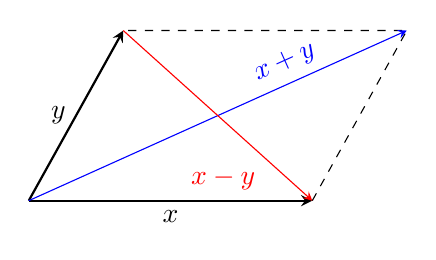
\begin{tikzpicture}[>=stealth, scale=1.2]
\coordinate (O) at (0,0);
\coordinate (X) at (3,0);
\coordinate (Y) at (1,1.8);
\coordinate (S) at (4,1.8);
\draw[dashed] (X) -- (S) -- (Y);
\draw[->, thick] (O) -- (X) node[midway, below] {$x$};
\draw[->, thick] (O) -- (Y) node[midway, left] {$y$};
\draw[->, blue] (O) -- (S) node[pos=0.7, above, sloped] {$x+y$};
\draw[->, red] (Y) -- (X) node[pos=0.75, below left] {$x-y$};
\end{tikzpicture}
\end{center}

\begin{theo}[Théorème de Pythagore]
\label{theo:pythagore-2}
Pour tous $x,y\in E$,
\[\ps{x}{y}=0\iff\|x+y\|^2=\|x\|^2+\|y\|^2\]
\end{theo}

\begin{proof}
D'après la proposition~\ref{prop:identites-remarquables}, $\|x+y\|^2-\|x\|^2-\|y\|^2=2\ps{x}{y}$, qui est nul si et seulement si $\ps{x}{y}=0$.
\end{proof}

\begin{remarque}
L'équivalence utilise que l'on travaille sur un $\mathbb{R}$-espace vectoriel : c'est la formule $\|x+y\|^2=\|x\|^2+\|y\|^2+2\ps{x}{y}$, propre au cas réel, qui donne le sens $(\Leftarrow)$.
\end{remarque}

\subsection{Inégalité de Cauchy--Schwarz}

\begin{theo}[Inégalité de Cauchy--Schwarz]
\label{theo:cauchy-schwarz}
Pour tous $x,y\in E$,
\[\big|\ps{x}{y}\big|\leq\|x\|\,\|y\|\]
avec égalité si et seulement si la famille $(x,y)$ est liée.
\end{theo}

\begin{proof}
Soient $x,y\in E$. Pour $\lambda\in\mathbb{R}$, posons
\[f(\lambda)=\ps{\lambda x+y}{\lambda x+y}=\|\lambda x+y\|^2\geq 0\]
D'après la proposition~\ref{prop:identites-remarquables} (appliquée à $\lambda x$ et $y$) et la proposition~\ref{prop:norme-associee-premieres},
\[f(\lambda)=\lambda^2\|x\|^2+2\lambda\ps{x}{y}+\|y\|^2\]

\textbf{Inégalité, premier cas : $x\neq 0$.} Alors $\|x\|^2>0$ (proposition~\ref{prop:norme-associee-premieres}), et $f$ est un trinôme du second degré, de discriminant
\[\Delta=4\ps{x}{y}^2-4\|x\|^2\|y\|^2\]
Évaluons $f$ en son sommet $\lambda_0=-\dfrac{\ps{x}{y}}{\|x\|^2}$ :
\[f(\lambda_0)=\frac{\ps{x}{y}^2}{\|x\|^2}-2\frac{\ps{x}{y}^2}{\|x\|^2}+\|y\|^2=\frac{\|x\|^2\|y\|^2-\ps{x}{y}^2}{\|x\|^2}=-\frac{\Delta}{4\|x\|^2}\]
Comme $f(\lambda_0)\geq 0$, on obtient $\Delta\leq 0$, c'est-à-dire $\ps{x}{y}^2\leq\|x\|^2\|y\|^2$. La fonction racine carrée étant croissante sur $[0,+\infty[$,
\[\big|\ps{x}{y}\big|=\sqrt{\ps{x}{y}^2}\leq\sqrt{\|x\|^2\|y\|^2}=\|x\|\,\|y\|\]

\textbf{Inégalité, second cas : $x=0$.} Alors $\ps{x}{y}=\ps{0}{y}=0$ (proposition~\ref{prop:ps-bilineaire}) et $\|x\|\,\|y\|=0$ : l'inégalité est vraie, et c'est même une égalité.

\textbf{Cas d'égalité, $(\Leftarrow)$.} Supposons $(x,y)$ liée : il existe $(\alpha,\beta)\neq(0,0)$ tel que $\alpha x+\beta y=0$.
\begin{itemize}
\item Si $\alpha\neq 0$, alors $x=\lambda y$ avec $\lambda=-\dfrac{\beta}{\alpha}$, et
\[\big|\ps{x}{y}\big|=\big|\ps{\lambda y}{y}\big|=|\lambda|\,\|y\|^2=\big(|\lambda|\,\|y\|\big)\|y\|=\|\lambda y\|\,\|y\|=\|x\|\,\|y\|\]
\item Si $\alpha=0$, alors $\beta\neq 0$ et $\beta y=0$, donc $y=0$ : $\big|\ps{x}{0}\big|=0=\|x\|\times 0$.
\end{itemize}

\textbf{Cas d'égalité, $(\Rightarrow)$.} Supposons $\big|\ps{x}{y}\big|=\|x\|\,\|y\|$.
\begin{itemize}
\item Si $x=0$, la famille $(x,y)$ est liée : $1\cdot x+0\cdot y=0$ avec $(1,0)\neq(0,0)$.
\item Si $x\neq 0$, l'égalité donne $\ps{x}{y}^2=\|x\|^2\|y\|^2$, c'est-à-dire $\Delta=0$, donc $f(\lambda_0)=0$ d'après le calcul ci-dessus. Ainsi $\|\lambda_0x+y\|^2=0$, d'où $\lambda_0x+y=0$ (proposition~\ref{prop:norme-associee-premieres}) : la famille $(x,y)$ est liée, avec les coefficients $(\lambda_0,1)\neq(0,0)$.\qedhere
\end{itemize}
\end{proof}

\begin{exemple}
\begin{itemize}
\item Dans $\mathbb{R}^n$ muni du produit scalaire canonique (exemple~\ref{ex:ps-canonique}) : pour tous réels $x_1,\dots,x_n,y_1,\dots,y_n$,
\[\left|\sum_{i=1}^nx_iy_i\right|\leq\sqrt{\sum_{i=1}^nx_i^2}\,\sqrt{\sum_{i=1}^ny_i^2}\]
\item Dans $\mathcal{C}([a,b],\mathbb{R})$ (exemple~\ref{ex:ps-integral}) : pour toutes $f,g$ continues sur $[a,b]$,
\[\left|\int_a^bf(x)g(x)\,\mathrm{d}x\right|\leq\sqrt{\int_a^bf(x)^2\,\mathrm{d}x}\,\sqrt{\int_a^bg(x)^2\,\mathrm{d}x}\]
\end{itemize}
\end{exemple}

\begin{theo}
\label{theo:norme-euclidienne}
L'application $\|\cdot\|:x\mapsto\sqrt{\ps{x}{x}}$ est une norme sur $E$ : $(E,\|\cdot\|)$ est un espace vectoriel normé.
\end{theo}

\begin{proof}
La positivité, la séparation et l'homogénéité ont été établies à la proposition~\ref{prop:norme-associee-premieres}. Il ne reste plus qu'à prouver l'inégalité triangulaire. Soient $x,y\in E$. D'après la proposition~\ref{prop:identites-remarquables} puis l'inégalité de Cauchy--Schwarz,
\begin{align*}
0\leq\|x+y\|^2&=\|x\|^2+\|y\|^2+2\ps{x}{y}\\
&\leq\|x\|^2+\|y\|^2+2\big|\ps{x}{y}\big|\\
&\leq\|x\|^2+\|y\|^2+2\|x\|\,\|y\|\\
&=\big(\|x\|+\|y\|\big)^2
\end{align*}
La fonction racine carrée étant croissante sur $[0,+\infty[$, et $\|x+y\|$, $\|x\|+\|y\|$ étant positifs, on obtient $\|x+y\|\leq\|x\|+\|y\|$.
\end{proof}

\begin{remarque}
La norme associée au produit scalaire canonique de $\mathbb{R}^n$ est la norme $\|\cdot\|_2$ de l'exemple~\ref{ex:normes-kn} : on vient donc de démontrer l'inégalité triangulaire pour $\|\cdot\|_2$, qui avait été admise, lorsque $K=\mathbb{R}$. Le cas $K=\mathbb{C}$ s'en déduit : pour $z,z'\in\mathbb{C}^n$, notons $|z|=(|z_1|,\dots,|z_n|)\in\mathbb{R}^n$, de sorte que $\|z\|_2=\||z|\|_2$. Comme $0\leq|z_i+z'_i|\leq|z_i|+|z'_i|$ pour tout $i$, on a $\|z+z'\|_2\leq\||z|+|z'|\|_2$ (les carrés des coordonnées sont rangés dans le même ordre), puis $\||z|+|z'|\|_2\leq\||z|\|_2+\||z'|\|_2=\|z\|_2+\|z'\|_2$ par le cas réel.
\end{remarque}

\begin{remarque}[Normes euclidiennes]
D'après la proposition~\ref{prop:identites-remarquables}, une norme associée à un produit scalaire vérifie l'identité du parallélogramme. Réciproquement, on admet qu'une norme $\|\cdot\|$ sur un $\mathbb{R}$-espace vectoriel est associée à un produit scalaire si et seulement si elle vérifie
\[\forall x,y\in E,\qquad\|x+y\|^2+\|x-y\|^2=2\big(\|x\|^2+\|y\|^2\big)\]
le produit scalaire étant alors nécessairement donné par l'identité de polarisation. Par exemple, sur $\mathbb{R}^2$, la norme $\|\cdot\|_\infty$ n'est associée à aucun produit scalaire : pour $x=(1,0)$ et $y=(0,1)$,
\[\|x+y\|_\infty^2+\|x-y\|_\infty^2=1+1=2\neq 4=2\big(\|x\|_\infty^2+\|y\|_\infty^2\big)\]
\end{remarque}

\section{Orthogonalité}

\subsection{Vocabulaire}

\begin{defi}[Vecteur unitaire]
\label{defi:unitaire}
Un vecteur $x\in E$ est dit \textbf{unitaire} si $\|x\|=1$.
\end{defi}

Pour tout $y\neq 0$, le vecteur $\dfrac{1}{\|y\|}\,y$ est unitaire, puisque $\left\|\dfrac{1}{\|y\|}y\right\|=\dfrac{1}{\|y\|}\,\|y\|=1$ (homogénéité). On dit qu'on \textbf{normalise} $y$ ; on définit ainsi une application
\[E\setminus\{0\}\to E\setminus\{0\},\qquad y\mapsto\frac{1}{\|y\|}\,y\]
En revanche, on ne peut pas rendre unitaire le vecteur nul : $\|\lambda\cdot 0\|=0$ pour tout $\lambda\in\mathbb{R}$.

\begin{defi}[Vecteurs orthogonaux]
\label{defi:orthogonaux}
Deux vecteurs $x,y\in E$ sont dits \textbf{orthogonaux} (entre eux) si $\ps{x}{y}=0$ ; on note alors $x\perp y$. Cette relation est symétrique.
\end{defi}

\begin{remarque}
Le vecteur nul est orthogonal à tout vecteur (proposition~\ref{prop:ps-bilineaire}), et c'est le seul vecteur orthogonal à lui-même (axiome 4).
\end{remarque}

\begin{defi}[Orthogonal d'une partie]
\label{defi:orthogonal-partie}
Soit $A$ une partie non vide de $E$. On appelle \textbf{orthogonal} de $A$ l'ensemble
\[A^\perp=\{x\in E\mid\forall a\in A,\ \ps{a}{x}=0\}\]
des vecteurs orthogonaux à tous les éléments de $A$.
\end{defi}

\begin{exemple}
$\{0\}^\perp=E$, puisque tout vecteur est orthogonal à $0$. À l'inverse, $E^\perp=\{0\}$ : si $x\in E^\perp$, alors en particulier $x\perp x$, donc $x=0$ ; et $0\in E^\perp$.
\end{exemple}

\begin{prop}
\label{prop:orthogonal-sev}
Soit $A$ une partie non vide de $E$. Alors $A^\perp$ est un sous-espace vectoriel de $E$.
\end{prop}

\begin{proof}
Par définition,
\[A^\perp=\bigcap_{a\in A}\Ker\big(\ps{a}{\cdot}\big)\]
Pour chaque $a\in A$, $\ps{a}{\cdot}$ est une forme linéaire sur $E$ (axiome 2), donc son noyau est un sous-espace vectoriel de $E$ : c'est un hyperplan si $a\neq 0$ (la forme est alors non nulle, puisque $\ps{a}{a}\neq 0$), et c'est $E$ tout entier si $a=0$. Une intersection de sous-espaces vectoriels de $E$ est un sous-espace vectoriel de $E$.
\end{proof}

\begin{defi}[Sous-espaces orthogonaux]
\label{defi:sev-orthogonaux}
Soient $F$ et $G$ deux sous-espaces vectoriels de $E$. On dit que $F$ et $G$ sont \textbf{orthogonaux}, et on note $F\perp G$, si
\[\forall (x,y)\in F\times G,\qquad\ps{x}{y}=0\]
autrement dit si $G\subset F^\perp$ (ou, de façon équivalente, $F\subset G^\perp$).
\end{defi}

\begin{prop}
\label{prop:orthogonaux-somme-directe}
Si $F\perp G$, alors la somme $F+G$ est directe.
\end{prop}

\begin{proof}
Soit $x\in F\cap G$. Comme $x\in F$, $x\in G$ et $F\perp G$, on a $\ps{x}{x}=0$, donc $x=0$. Ainsi $F\cap G=\{0\}$, et la somme est directe (proposition~\ref{prop:somme-directe-deux}).
\end{proof}

\begin{prop}
\label{prop:double-orthogonal}
Soit $A$ une partie non vide de $E$. Alors $A\subset(A^\perp)^\perp$.
\end{prop}

\begin{proof}
L'ensemble $A^\perp$ est non vide (c'est un sous-espace vectoriel, il contient $0$), donc
\[(A^\perp)^\perp=\{x\in E\mid\forall b\in A^\perp,\ \ps{b}{x}=0\}\]
est bien défini, et c'est un sous-espace vectoriel de $E$ (proposition~\ref{prop:orthogonal-sev}). Soit $a\in A$. Pour tout $b\in A^\perp$, on a $\ps{a}{b}=0$ par définition de $A^\perp$, donc $\ps{b}{a}=0$ par symétrie. Ainsi $a\in(A^\perp)^\perp$.
\end{proof}

\begin{exemple}[Un hyperplan d'orthogonal nul]
\label{ex:hyperplan-orthogonal-nul}
Soit $E=\mathbb{R}[X]$. Pour $P=\sum_{i\geq 0}p_iX^i$ et $Q=\sum_{i\geq 0}q_iX^i$ (les coefficients étant nuls à partir d'un certain rang), on pose
\[\ps{P}{Q}=\sum_{i=0}^{+\infty}p_iq_i\]
(la somme ne porte en fait que sur un nombre fini de termes non nuls). Soit $F=\{P\in\mathbb{R}[X]\mid P(1)=0\}$. Alors :
\begin{enumerate}
\item $\langle\cdot\mid\cdot\rangle$ est un produit scalaire sur $\mathbb{R}[X]$ ;
\item $F$ est un hyperplan de $\mathbb{R}[X]$ ;
\item $F^\perp=\{0\}$.
\end{enumerate}
En particulier $F\oplus F^\perp=F\neq E$ : en dimension infinie, l'orthogonal d'un sous-espace n'en est pas toujours un supplémentaire. De plus $(F^\perp)^\perp=\{0\}^\perp=E\neq F$ : l'inclusion de la proposition~\ref{prop:double-orthogonal} peut être stricte.
\end{exemple}

\begin{proof}
\textbf{1.} La symétrie est claire ($p_iq_i=q_ip_i$). Les coefficients de $\lambda Q+R$ sont les $\lambda q_i+r_i$, d'où la linéarité à droite comme pour le produit scalaire canonique de $\mathbb{R}^n$. On a $\ps{P}{P}=\sum_ip_i^2\geq 0$, et si $\sum_ip_i^2=0$, alors pour tout $i\in\mathbb{N}$, $0\leq p_i^2\leq\sum_jp_j^2=0$, donc $p_i=0$ : $P=0$.

\textbf{2.} \emph{Première méthode.} L'évaluation $\mathrm{ev}_1:P\mapsto P(1)$ est une forme linéaire sur $\mathbb{R}[X]$, non nulle puisque $\mathrm{ev}_1(1)=1$ ; donc $F=\Ker(\mathrm{ev}_1)$ est un hyperplan.

\emph{Seconde méthode.} Montrons que $F\oplus\Vect(1)=\mathbb{R}[X]$. Tout $P\in\mathbb{R}[X]$ s'écrit $P=\big(P-P(1)\big)+P(1)$, avec $P-P(1)\in F$ et $P(1)\in\Vect(1)$. Et si un polynôme constant $c$ appartient à $F$, alors $c=c(1)=0$ : $F\cap\Vect(1)=\{0\}$.

\textbf{3.} Un polynôme $Q$ appartient à $F$ si et seulement si $1$ est racine de $Q$, c'est-à-dire si et seulement s'il existe $T=\sum_{n\geq 0}t_nX^n\in\mathbb{R}[X]$ tel que $Q=(X-1)T=\sum_{n\geq 0}t_n(X-1)X^n$. Ainsi
\[F=\Vect\big((X-1)X^n\big)_{n\in\mathbb{N}}\]
(cette famille est d'ailleurs libre, car formée de polynômes de degrés deux à deux distincts : c'est une base de $F$).

Soit $P=\sum_ip_iX^i\in F^\perp$. Pour tout $n\in\mathbb{N}$, $(X-1)X^n=X^{n+1}-X^n\in F$, donc
\[0=\ps{X^{n+1}-X^n}{P}=p_{n+1}-p_n\]
La suite $(p_n)_{n\in\mathbb{N}}$ est donc constante, égale à $p_0$. Or $P$ est un polynôme : il existe $N\in\mathbb{N}$ tel que $p_N=0$, d'où $p_0=p_N=0$, puis $p_n=0$ pour tout $n$ : $P=0$. Ainsi $F^\perp\subset\{0\}$, et l'inclusion réciproque est vraie car $F^\perp$ est un sous-espace vectoriel.

Enfin $F^\perp=\{0\}$ donne $F\oplus F^\perp=F\oplus\{0\}=F$, qui est différent de $E$ puisque $1\notin F$.
\end{proof}

\subsection{Familles orthogonales et orthonormales}

\begin{defi}[Famille orthogonale, orthonormale]
\label{defi:famille-orthonormale}
Une famille $(e_i)_{i\in I}$ de vecteurs de $E$ est dite :
\begin{itemize}
\item \textbf{orthogonale} si ses vecteurs sont deux à deux orthogonaux : $\forall(i,j)\in I^2,\ i\neq j\implies\ps{e_i}{e_j}=0$ ;
\item \textbf{orthonormale} si $\forall(i,j)\in I^2,\ \ps{e_i}{e_j}=\delta_{i,j}$, où $\delta_{i,j}$ vaut $1$ si $i=j$ et $0$ sinon ; autrement dit, si elle est orthogonale et formée de vecteurs unitaires.
\end{itemize}
En particulier, une famille orthonormale est orthogonale.
\end{defi}

\begin{exemple}
La base canonique de $\mathbb{R}^n$ est orthonormale pour le produit scalaire canonique. La famille $(X^n)_{n\in\mathbb{N}}$ est orthonormale pour le produit scalaire de l'exemple~\ref{ex:hyperplan-orthogonal-nul}.
\end{exemple}

\begin{prop}
\label{prop:orthonormale-libre}
Toute famille orthonormale est libre.
\end{prop}

\begin{proof}
Soit $(e_i)_{i\in I}$ une famille orthonormale. Soient $J\subset I$ une partie finie et $(\alpha_j)_{j\in J}\in\mathbb{R}^J$ tels que $\sum_{j\in J}\alpha_je_j=0$. Pour tout $i\in J$, par linéarité à gauche,
\[0=\ps{0}{e_i}=\Ps{\sum_{j\in J}\alpha_je_j}{e_i}=\sum_{j\in J}\alpha_j\ps{e_j}{e_i}=\sum_{j\in J}\alpha_j\delta_{j,i}=\alpha_i\]
Tous les $\alpha_i$ sont nuls : la famille est libre.
\end{proof}

\begin{remarque}
Plus généralement, toute famille orthogonale de vecteurs \emph{non nuls} est libre : le même calcul donne $0=\alpha_i\|e_i\|^2$, avec $\|e_i\|^2\neq 0$, donc $\alpha_i=0$. L'hypothèse « non nuls » est nécessaire : la famille $(0)$ est orthogonale mais liée.
\end{remarque}

\begin{theo}[Théorème de Pythagore]
\label{theo:pythagore}
Si $(e_1,\dots,e_k)$ est une famille orthogonale de vecteurs de $E$, alors
\[\left\|\sum_{i=1}^ke_i\right\|^2=\sum_{i=1}^k\|e_i\|^2\]
\end{theo}

\begin{proof}
Par développement bilinéaire (proposition~\ref{prop:developpement-bilineaire}),
\[\left\|\sum_{i=1}^ke_i\right\|^2=\Ps{\sum_{i=1}^ke_i}{\sum_{j=1}^ke_j}=\sum_{i=1}^k\sum_{j=1}^k\ps{e_i}{e_j}=\sum_{i=1}^k\ps{e_i}{e_i}=\sum_{i=1}^k\|e_i\|^2\]
car, la famille étant orthogonale, seuls les termes d'indices $i=j$ sont éventuellement non nuls.
\end{proof}

\begin{remarque}
Pour $k=2$, c'est le sens direct du théorème~\ref{theo:pythagore-2}, qui est une équivalence. Pour $k\geq 3$, la réciproque est fausse : dans $\mathbb{R}^2$ muni du produit scalaire canonique, avec $e_1=(1,0)$, $e_2=(0,1)$, $e_3=(1,-1)$, on a $e_1+e_2+e_3=(2,0)$ et
\[\|e_1+e_2+e_3\|^2=4=1+1+2=\|e_1\|^2+\|e_2\|^2+\|e_3\|^2\]
alors que $\ps{e_1}{e_3}=1\neq 0$.
\end{remarque}
